%% document class
\documentclass[10pt,oneside,leqno,openright]{memoir}

\input{macros}
\newcommand*{\sto}{\rightsquigarrow}


\begin{document}

\frontmatter
\thispagestyle{empty}
\begin{center}
  \LARGE
  {\bfseries Synthetic Homotopy Theory}\\[1cm]
  \large Abbreviated lecture notes\\[5mm]
  \Large Midlands Graduate School (MGS)\\
  \large 13--17 April 2026, Nottingham, UK\\[1cm]
  by\\
  Axel Ljungström and Aref Mohammadzadeh\\
  School of Computer Science\\
  University of Nottingham\\[1cm]
  Heavily based on notes from MGS 2024 by
  Ulrik Buchholtz and Mark Williams\\
  %\Large NB\enspace Subject to change: Refresh if needed
\end{center}

\vfill

%\begin{abstract}
%  These lecture notes aim to introduce the field of synthetic homotopy theory to a (mainly) computer science audience. That is, we shall assume that the reader cares about types,
%\end{abstract}

\clearpage

%\tableofcontents*

\mainmatter

%% \setcounter{chapter}{-1}

%% \chapter{Introduction}




\chapter*{Lecture 1}
%\textcite{Shulman-logic-of-space}
\subsection*{What is homotopy theory?}
Homotopy theory is the study of paths between.
\subsection*{What is synthetic homotopy theory?}
Synthetic homotopy theory is the study of the identity type in Martin-Löf Type Theory.
\subsection*{What is the connection?}
Awodey, Hoffmann, Streicher, Voevodsky, Warren\footnote{Voevodsky is the person who is directly attributed this connection, but the other authors have also made crucial contributions that inspired this interpretation}:
\begin{itemize}
\item \axel{Turns out: types in type theory can be interpreted as spaces}
  \begin{itemize}
  \item `A is a type' (or $A : \UU$) ---> `$A$ is a topological space (up to \emph{homotopy}, i.e.\ continuous deformation, but we don't need to worry about this now)'
  \item $x:A$ ---> `$x$ is a point in $A$. 
  \item $p:x=_Ay$ ---> `$p$ is a (continuous) path from $x$ to $y$ in $A$'.
  \item $r: p=_{x= y}q$ ---> `$p$ is a \emph{higher} path/continuous deformation/\emph{homotopy} from $p$ to $q$'
  \end{itemize}
\end{itemize}
\begin{center}
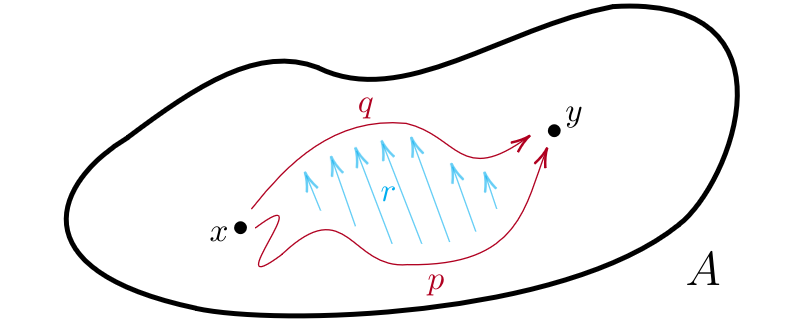
\includegraphics[scale=.2]{my_space.png}
\end{center}

While all paths may be interesting to homotopy theorists, there are certainly quite a lot of them... One thing that homotopy theorists like to do is to restrict to a certain classs of paths, namely those that are \emph{loops}, i.e.\ start and end on the same point.

\[\text{\axel{Draw pic}}\]

Given a space $A$ and $x\in A$, we can define
\[\pi_1(A,x) := \{\text{Loops in $A$ starting and ending at x}\} / \sim \]
where we quotient out by \emph{homotopy} -- two loops are equal if one can be continuously deformed into the other. The reason that we restrict to loops is that this gives us a group structure. Indeed, given two loops $p$ and $q$, we can compose these (`walk along $p$ and then along $q$'). Similarly, we can revert them: $p^{-1} = \textit{`$p$, but backwards'}$. We also get a neutral element $\mathsf{const}_x$ which is the constant loop standing still on $x$.

The group $\pi_1(A,x)$ is called the \emph{fundamental group} of $A$
(based at $x$). Now, why stop at $1$-dimensional loops from $x$ to
itself? We can easily (although we won't do it here) define the notion
of an $n$-dimensional loop and can similarly define
%
\[\pi_n(A,x) = \{\text{$n$-dimensional loops in $A$ touching $x$}\}/\sim \]
%
where we again quotient by an appropriate notion of homotopy.
%
This is called the \emph{$n$th homotopy group of $A$ (based at $x$)}.
%
Knowing $\pi_n(A,x)$ a space $A$ and suitable $x \in A$ for all $n$ esentially tells you `all you need to know' about your space (if you're a homotopy theorist, that is).
%
Unfortunately, these are \emph{incredibly hard} to compute in general.
%
For this reason, homotopy theorists often focus on the special case when $A$ is the $m$-dimensional (hyper-)sphere $S^m$.
%
In a way, all spaces can (`up to homotopy') be thought of as consisting of a bunch of spheres of varying dimension glued together, this seems like a very suitable thing to study.
%
Unfortunately, also computing $\pi_n(S^m,\star)$ for arbitrary $n,m \geq 1$ is notoriously hard -- or perhaps this is fortunate, since computing these has, in a way, become the raison d'etre of homotopy theory.

The goal of this course will be to explore whether we can compute any of these $\pi_n(S^m,\star)$ in synthetic homotopy theory, i.e.\ using the language of dependent type theory or, actually, \emph{Homotopy Type Theory} (HoTT), an extension of this language). In thislecture, we will define homotopy groups in HoTT. In lecture 2, we introduce some actual spaces into our type theory (in particular spheres). In lectures 3 and 4 we will compute some homotopy groups of these spaces -- in particular of the circle and the $3$-sphere.

Note, that HoTT is just dependent type theory with \emph{univalence} and \emph{higher inductive types}. I'll introduce these concepts as we go. 



\section*{Paths}
Let us recall what is probably the most important notion from dependent type theory:
\begin{definition}[Path induction]
  Let $x:A$. In order to prove a statement/construct an element of type $(y:A) (p : x = y) \to B(y,p)$, it suffices to prove/construct an element of $B(x,\refl_x)$.
 \end{definition}
%
Let's give some examples of this principle in action:
%
\begin{example}[Transport]
  Given $p: x =_A y$ and $B:A \to \UU$, we get a map $\trp^B_p : B(x) \to B(y)$ by path induction on $p$:
  \[\trp^B_{\refl_{x}} : B(x) \to B (x) \quad := \quad \mathsf{id}_{B(x)}\]
\end{example}
%
\[\text{\axel{draw picture explaining transport}}\]

\begin{example}[Function application]
  Given $f :X \to Y$ and $p:x=y$, we have $\ap_f(p) : f(x) = f(y)$ (by path induction on $p$).
\end{example}

\paragraph{Question.} Function application is only stated for plain functions, but we're in dependent type theory. What if $f : (x:X) \to B(x)$ is a dependent function?

We can't write $\ap_f(p) : f(x) = f(y)$ because $f(x) : B(x)$ and $f(y):B(y)$, so this equality doesn't type check! But $B(x)$ and $B(y)$ are equal types (by $p$), so we should still be able to express the idea that $f(x)$ and $f(y)$ are `equal' (modulo $p$):

\begin{definition}[Dependent paths]
  Given $B: X \to \UU$ dep. type, $p: x_0 = x_1$, and terms $b_0 : B(x_0)$ and $b:B(x_1)$, define
  \[(b_0 =^B_p b_1) := (\trp^B_p(b_0) = b_1) \]
\end{definition}

Note that the above definition coincides \emph{exactly} with the usual identity type whenever $p$ is $\refl$.

\begin{example}[Function application]
  Given $f :X \to Y$ and $p:x=y$, we have $\apd_f : (p : x = y) \to f(x) =^B_p f(y)$ (by path induction on $p$).
\end{example}

Remember that homotopy theorists were interested in composing paths and inverting paths? In HoTT, this idea simply corresponds to the fact that our identity type is transitive and symmetric.

\begin{example}[Path composition/inversion]
  Given $p: x = y$ and $q:y = z$, we can define $p\cdot q : x = z$ and $p^{-1} : y = z$ by path induction on $p$. These operations satisfy (for suitable $p$, $q$ and $r$):
\begin{itemize}
\item $p \cdot p^{-1} = \refl$
\item $p^{-1} \cdot p = \refl$
\item $p \cdot \refl = p$
\item $\refl \cdot p = p$
\item $(p \cdot q) \cdot r = p \cdot (q \cdot r)$
\end{itemize}
 \end{example}

\subsection*{Are we there yet?}
So, we have path types with notions of composition, inversion, and a neutral element. Why not just play the same game as in traditional homotopy theory and set $\pi_1(X,x) := (x = x)$ with group operations given by path composition and path reversal.
%
This is \emph{almost} right. The issue: the group laws hold but they
can hold in \emph{infinitely many ways}! Suppose you and I both are
tasked with defining $\pi_1(X,x)$ in type theory. Both of us provide
the same underlying type, the same operations, and the same neutral
element -- but we have provided different proofs of the fact that,
say, $p \cdot p^{-1} = \refl$. Which definition is the appropriate
one? Mine or yours? To arrive at a well-defined notion of groups, we
would like to make sure that this situation never arises -- we would
like to `quotient' by all `higher paths' (i.e. paths involving other
paths, such as the path witnessing $p\cdot p^{-1} = \refl$.
%
The next part of this lecture is about how to construct these kinds of quotients.

\section*{$n$-types}
In order to even state that we wish to `quotient out higher paths', we need a way to pinpoint what we even mean by `higher paths'. A good way of capturing a type having `higher structure' in general is the notion of an $n$-type.  Let us start with two special cases:
%
\begin{definition}
    A type $X$ is \textbf{contractible} if the type
    \[ \isContr(X) := (x : X) \times ((y : X) \to x =_X y) \]
    is inhabited.
\end{definition}
%
\begin{definition}
    A type $X$ is a \textbf{proposition} if the type
    \[ \isProp(X) := (x, y : X) \to x =_X y\]
    is inhabited.
\end{definition}
%
Usin this, we can define what it means to be an $n$-type:
\begin{definition}
    A type $X$ is
    \begin{itemize}
        \item a \textbf{($-2$)-type} if $\isContr{A}$,
        \item a \textbf{($-1$)-type} if $\isProp{A}$, and
        \item an \textbf{$n$-type} if $(x, y : X) \to \isType{(n-1)}(x=_Ay)$.
    \end{itemize}
\end{definition}
We may use the following conventions
\begin{convention}\phantom{.}
  \begin{itemize}
  \item $0$-types are called \textbf{Sets}
  \item $1$-types are called \textbf{Groupoids}
  \end{itemize}
\end{convention}
To get some intuition (hopefully, you will get even more later on in the course), let us give some `concrete' examples.
\begin{example}\phantom{.}
  \begin{itemize}
  \item All $(-2)$-types:
    \begin{itemize}
      \item The unit type $1$. Actually, all $(-2)$-types are equivalent to this type.
      \item The \textbf{singleton} type (over some $x:X$) i.e.\ $(y : X) \times (x = y)$ is contractible.
    \end{itemize}
  \item Propositions ($(-1)$-types):
    \begin{itemize}
    \item $1$, $\emptyset$ (and everything in between)
    \item The statement that a type is an $n$-type is itself a $(-1)$-type: $\mathsf{isProp}(\isType{n}(X))$.
    \item We haven't come this far yet, but we will soon define what it means for a function to the an equivalence (roughly, `invertible'). The statement that $f: A \to B$ is an equivalence is a $(-1)$-type.
    \end{itemize}
  \item Sets ($0$-types). These are types that are discrete in nature -- they can have a bunch of points but no interesting paths (i.e.\ no interesting homotopical structure):
    \begin{itemize}
    \item Any (plain) inductive type, e.g.\ $\bZ$
    \item cf. Hedberg's theorem if you're interested in how to prove this
    \end{itemize}
  \item $n$-type:
    \begin{itemize}
    \item The universe of $n$-types, $\UU^{\le n} := (X : \UU) \times \isType{n}(X)$, is an $(n+1)$-type.
    \item Any $n$-type is also an $(n+1)$-type.
    \end{itemize}
  \end{itemize}
\end{example}

%% \begin{remark}
%%     We call $0$-types sets and $1$-types groupoids. These correspond exactly to the usual notions!
%%     This also explains the indexing, as sets are \say{$0$-dimensional} objects. But it's also natural to use an indexing where contractible types are at level $0$: This hierarchy is called the h-level (homotopy level) hierarchy, so a type is \textbf{of hlevel $n+2$} if and only if it is an $n$-type.
%% \end{remark}

\begin{example}
We give some basic examples of $n$-types.
\begin{itemize}
\item The only $-2$-type is the unit type $1$. More precisely, the type of
  $-2$-types is contractible.
  \begin{itemize}
    \item Important mention: the \textbf{singleton} type (over some $x:X$) i.e. $(y : X) \times (x = y)$ is contractible.
  \end{itemize}
    \item $-1$-types are subtypes of $1$. For example the empty type $0$.
    \item The type of integers $\ZZ$ is a $0$-type. More generally any (non higher) inductive type is a $0$-type.
    \item The type of $n$-types in a universe $\UU$, $\UU^{\le n}$, is an $n+1$ type, for $n\ge-1$.
    \item Any $n$-type is also an $(n+1)$-type
\end{itemize}
\end{example}

We said before that we'd like to be able to `quotient' by all `higher
structure' of a type.
%
In other words, we would like to be able to take a type and turn it into an $n$-type.
%
This is precisely the role of the $n$-truncation.
%
Here, it is stated as a definition, although we never show how it's defined... For now, take it for granted:
\begin{definition}
  Given a type $X$, there is an $n$-type $\Trunc{X}_n$ equipped with a map $\trunc{-}_n: X \to \Trunc{X}_n$ s.t. for every $f: X \to Y$ where $Y$ is an $n$-type, we have
\[\begin{tikzcd}[ampersand replacement=\&]
	X \& Y \\
	{\Trunc{X}_n}
	\arrow["f", from=1-1, to=1-2]
	\arrow["{\trunc{-}_n}"', from=1-1, to=2-1]
	\arrow[dashed, from=2-1, to=1-2]
\end{tikzcd}\]
\textbf{Alternatively:}
    \[\blank\circ\trunc\blank_n : (\Trunc X_n \to Y) \to (X \to Y)\] is an
equivalence.
This phrasing might be better because we easily are able to generalise it to get the induction principle (i.e. dependent elimination) for any dependent ($n$-)type $B : X \to \UU^{\le n}$: we require that
\[\blank\circ\trunc\blank_n : ((x : \Trunc X_n) \to B(x)) \to ((x:X) \to B(\trunc{x}_n))\]
is an equivalence.
\end{definition}
\begin{itemize}
  \item Common notation: $\Trunc{X} := \Trunc{X}_{-1}$
\end{itemize}


\section*{Finally: Homotopy groups}

\begin{definition}
    A \textbf{pointed type} is a pair $(X, \star_X) : \ub{\UU_\star}{(X : \UU) \times X}$ where $X : \UU$ and $\star_X : X$.
\end{definition}
\begin{definition}
  A \textbf{pointed map} is a pair $(f ; \star_X) : \ub{(X,\star_X) \to_\star (Y,\star_Y)}{(f : X \to Y) (\times f(\star_X) = \star_Y)}$
\end{definition}
\begin{notation}\phantom{.}
  \begin{itemize}
  \item Often simply write $X : \UU_\star$ and $f : X \to_\star Y$, i.e.\ we leave basepoints and pointedness proofs implicit
  \item Always write $\star_X : X$ for basepoints and $\star_f : f(\star_X) = \star_Y$ for pointedness proofs. 
  \end{itemize}
\end{notation}

\begin{definition}
    We define the \textbf{loop space} of a pointed types $X$ by
    \[ \Omega(X) := (\star_X = \star_X)\]
This type is itself pointed by $\refl_{\star_X}$.
\end{definition}

\begin{itemize}
  \item It is \textbf{functorial}: given $f : X \to_\star Y$, we define $\Omega(f) : \Omega(X) \to \Omega(Y)$ by
    \[\Omega(f)(p) := (\star_f)^{-1} \cdot \ap_f(p) \cdot \star_f\]
  \item Path composition defines a `group structure' on $\Omega$
    \begin{itemize}
    \item Problem: group laws only hold up to homotopy.
      \begin{itemize}
      \item For instance there might be more than one element of $p \cdot p^{-1} = \refl_{\star_X}$.
      \end{itemize}
    \item Solution: need to truncate
    \end{itemize}
\end{itemize}

\begin{definition}
  The \textbf{first homotopy group} of a pointed type $X$ is defined by $\pi_1(X):= \Trunc{X}_0$
  \begin{itemize}
    \item Multiplication is inherited immediately from path composition on $\Omega(X)$. By the univeral property: $\trunc{p}_0 \cdot \trunc{q}_0 = \trunc{p \cdot q}_0$
  \end{itemize}
\end{definition}

\paragraph{Note} $\Omega : \UU_\star \to \UU_\star$ -- can be iterated.

\begin{definition}
    The $n$th homotopy group of $X:\UU_\star$ is defined by
    \[ \pi_n X := \setTrunc{\Omega^n X}\]
    Note that $n \geq 1$!
\end{definition}
\begin{itemize}
\item $\Omega$ is functorial $\implies$ $\pi_n$ is functorial
\item Write $f^* := \pi_n(f) : \pi_n(X) \to \pi_n(Y)$ for its functorial action.
\end{itemize}




\section{Things I should've talked about but didn't}
I didn't have time to mention that there is a notion of $n$-connected types. This notion is, in a sense, dual to the notion of $n$-type:
\begin{definition}
    A type $X$ is \textbf{$n$-connected} if $\Trunc{X}_n$ is contractible.
\end{definition}
We often simply write `connected' instead of `$0$-connected'.
\begin{proposition}
  If $X$ is $(n \geq -1)$-connected, then $x=_{X}y$ is $(n-1)$-connected for all $x,y:X$.
\end{proposition}

Just like types and and functions 
\begin{definition}
  The \textbf{fibre} of a function $f:X\to Y$ over a point $y : Y$ is the type
  \[ \fib_f(y) := (x : X) \times (f(x) = y) \]
\end{definition}

\begin{definition}
    A map $f : X \to Y$ is:
    \begin{enumerate}
        \item \textbf{$n$-truncated} if $\fib_f(y)$ is an $n$-type for all $y:Y$,
        \item \textbf{$n$-connected} if $\fib_f(y)$ is $n$-connected for all $y:Y$.
    \end{enumerate}
\end{definition}

%% As special cases, a map $f:X\to Y$ is \textbf{surjective} if it's $-1$-connected
%% and an \textbf{embedding} if it's $-1$-truncated. For reasons we'll see later, we think of $0$-truncated maps as \textbf{set bundles}.
%% \begin{example}
%%     The map $\trunc{\blank}_n : X \to \Trunc{X}_n$ is $n$-connected.
%% \end{example}



  


\axel{Let's compute some very exciting homotopy groups!}
\begin{proposition}
  If $X$ is an $n$-type, then $\pi_{k}(X)$ vanishes $\forall k>n$.
\end{proposition}
\begin{corollary}
  $\pi_{n \geq 1}(X)$ vanishes for any set $X$. In particular for $X = 1$.
\end{corollary}
\begin{proposition}
  If $X$ is $n$-connected, then $\pi_{k}(X)$ vanishes $\forall k\leq n$.
\end{proposition}

\subsection*{Recap: univalence}
\begin{definition}
  A function $f:X\to Y$ is an \textbf{equivalence} if $\fib_f(y)$ is contractible for all $y$.
\end{definition}
\begin{itemize}
\item Let $(X\simeq Y) \times \isEquiv(f)$
\item Fact: $\id_X : X \to X$ is an equivalence.
\end{itemize}

\begin{remark}\label{rmk:qinv}
  Why not use $\underset{:= \qinv(f)}{\underbrace{(g : (Y \to X)) \times (g \circ f = \id) \times (f \circ g = \id)}}$ as definition?
  \begin{itemize}
  \item \axel {Too much structure}
  \item $\qinv(f) \leftrightarrow \isEquiv(f)$ but $\qinv(f) \not\simeq \isEquiv(f)$. \axel{For our purposes, we can pretend that they are the same}.
  \end{itemize}
\end{remark}

\begin{axiom}[Univalence]
  The canonical map $X=_\UU Y \to (X \simeq Y)$ is an equivalence.
\end{axiom}

\begin{itemize}
\item In particular, $X \simeq Y \to X = Y$
\end{itemize}

\begin{fact}
  Univalence $\implies$ $\funExt(f) := (((x y : X) \to f(x) = g(x)) \to f = g)$
\end{fact}

\begin{itemize}
\item From now on, always assume univalence (and funExt). 
\end{itemize}




%% More exciting:
%% \begin{proposition}
%%   If $X$ is $n$-connected, then $\pi_{k}(X)$ vanishes $\forall k\leq n$.
%% \end{proposition}
%% \begin{proposition}
%%   Let $f : X \to_\star Y$ be $n$-connected. Then $f^* : \pi_k(X) \to \pi_k(Y)$ is
%%   \begin{itemize}
%%   \item an isomorphism when $k \leq n$,
%%   \item surjective when $k = n+1$ and
%%   \end{itemize}
%% \end{proposition}
%% \begin{itemize}
%%   \item $\uparrow$ key tool for computing homotopy groups of highly connected spaces, e.g.\ $n$-\textbf{spheres}.
%% \end{itemize}

%% \section*{Digression: the fundamental theorem of identity types}

%% \begin{itemize}
%% \item Understanding homotopy groups = understanding identity types
%% \item These are uniquely characterised by $\refl$ and path induction. Formally:
%% \end{itemize}
%% %
%% \begin{theorem}[The Fundamental Theorem of Identity Types]
%%     Let $R : X \to X \to \UU$ be a reflexive binary relation. The following are equivalent   \begin{enumerate}
%%         \item The obvious map\footnote{i.e.\ the map defined by path induction which
%%           sends $\refl_x$ to the term of type $R(x,x)$ given to us by
%%           reflexivity of $R$} $x =_A y \to R(x,y)$  is an equivalence.
%%         \item For any $x :X$, the total space $(y : X) \times (R(x ,y))$ is contractible.
%%     \end{enumerate}
%% \end{theorem}

%% \begin{example}
%%   \textbf{Q.} Given $(x,y) ,(x',y') : (x:X)\times B(x)$, how can we describe
%%   \[(x,y) =_{(x : X) \times B(x)} (x',y')?\]
%%   %
%%   \textbf{A.} Define $R : \left[(x:X)\times B(x) \right]^2 \to \UU$ by
%%   \[R((x,y),(x',y')) := (p : x = y) \times (x' =^B_p y')\]
%%   and show that
%%   \[\left[(x',y') : (x :X ) \times B(x)\right] \times R((x,y),(x',y'))\] is contractible:
%% \begin{align*}
%%   &\left[(x',y') : (x :X ) \times B(x)\right] \times R((x,y),(x',y')) \\
%%   \simeq\;
%%   & \ub{\mathsf{contr}}{(x': X) \times (p : x = x')} \times (y' : B(x')) \times (y =^B_p y') \\
%%   \simeq\;
%%   &(y':B(x))\times(y = y')
%%   \simeq 1
%% \end{align*}
%% %
%% \end{example}
%% Pointed version:
%% %
%% \begin{theorem}[The Fundamental Theorem of Identity Types]
%%   Let $X$ be a pointed type and $Y: X \to \UU$ a family of types equipped with a point $y_0 : (\star_X)$. The following statments are equivalent:
%%   \begin{enumerate}
%%         \item The obvious map $\star_X =_A x \to Y(x)$  is an equivalence.
%%         \item The total space $(x : X) \times Y(x)$ is contractible.
%%     \end{enumerate}
%% \end{theorem}
%
%% This in turn can be used to establish the following important characterization of type families,
%% sometimes known as \textbf{straightening--unstraightening}.
%% \begin{theorem}
%%   For any small type $X:\UU$, forming the dependent sum along with the first projection gives an equivalence:
%%   \[
%%     (X \to \UU) \simeq \Bigl((Y : \UU) \times (Y \to X)\Bigr)
%%   \]
%% \end{theorem}
%% The inverse maps a type over $X$, $f : Y\to X$, to the family of fibers, $\fib_f$.
%% %
%% Let us spell out the key consequence of this theorem, because it is \emph{incredibly useful}. Fix a predicate $P : (X : \UU) \times (X \to Y) \to \UU$, i.e.\ a statement about universally quantified over all types $X$ and maps $X \to Y$. In order to prove that $P(X,f)$ holds for all $X \rightarrow{f} Y$, it suffices to prove $P$ for all first projections of the form $(y:Y) \times B(y) \xrightarrow{\fst} Y$.  

%% \section{Exercises}
%% \begin{enumerate}
%%     \item Show that for $n \geq m$ and any type $A$ we have
%%     \[ \Trunc{\Trunc{A}_n}_m \simeq \Trunc{A}_m. \]

%%   \item\label{ex:n-conn-orth}
%%     Show that a type $X$ is $n$-connected if and only if, for every $n$-type $Y$,
%%     the diagonal map
%%     \[ Y \to (X \to Y), \quad y\mapsto (x\mapsto y),
%%     \]
%%     is an equivalence.

%%   \item Show that the map $\trunc\blank_n : X \to \Trunc X_n$ is $n$-connected.

%%     \item Consider a map $f : X \to Y$.
%%       We define its \textbf{$n$-image} to be the type $\im_n(f) :=
%%       (y : Y) \times \Trunc{\fib_f(y)}_n$.
%%     \begin{enumerate}
%%     \item Show that we can factorise $f$ through the $n$-image, that is,
%%       construct a commuting diagram:
%%         \[\begin{tikzcd}
%%             X \ar[rr, "f"] \ar[dr, swap, "p"] & & Y \\
%%             & \im_n(f) \ar[ur, swap, "i"]
%%         \end{tikzcd}\]
%%     \item Show that $p$ is $n$-connected and $i$ is $n$-truncated.
%%     \item Show that if $Z$ is any type, $g : X \to Z$ is $n$-connected, and $h:Z\to Y$ is $n$-truncated with $f = h\circ g$, then there is a unique equivalence $e : \im_n(f) \to Z$ with $e\circ p = g$ and $h\circ e = i$:
%%       \[
%%         \begin{tikzcd}
%%       & Z \ar[dr,"h"] & \\
%%       X \ar[rr,pos=0.7,"f"]\ar[dr,"p"'] \ar[ur,"g"]& & Y\\
%%       & \im_n(f)\ar[ur,"i"']\ar[uu,dotted,pos=0.3, "e"] &
%%     \end{tikzcd}
%%   \]
%%   (\emph{Hint})\enspace It's easier if you assume $g$ and $h$ are projections of
%%   dependent sums.
%%     \end{enumerate}

%%     \item (Eckmann--Hilton). All paths will take place in a fixed type $X$.
%%     \begin{enumerate}
%%         \item Given paths $p_0, p_1 : x = y$ and $q_0, q_1: y = z$, and higher paths $r : p_0 = p_1$ and $s : q_0 = q_1$, define their \textbf{horizontal multiplication} $s \ast r : q_0 \cdot p_0 = q_1 \cdot p_1$ by path induction on $r$ and $p_0$.
%%         \[\begin{tikzcd}
%%     	x & y & z
%%     	\arrow[""{name=0, anchor=center, inner sep=0}, "{p_1}"', bend right=40, from=1-1, to=1-2]
%%     	\arrow[""{name=1, anchor=center, inner sep=0}, "{q_1}"', bend right=40, from=1-2, to=1-3]
%%     	\arrow[""{name=2, anchor=center, inner sep=0}, "p_0", bend left=40, from=1-1, to=1-2]
%%     	\arrow[""{name=3, anchor=center, inner sep=0}, "q_0", bend left=40, from=1-2, to=1-3]
%%     	\arrow["s", shorten <=3pt, shorten >=3pt, Rightarrow, from=3, to=1]
%%     	\arrow["r"', shorten <=3pt, shorten >=3pt, Rightarrow, from=2, to=0]
%%         \end{tikzcd}\]

%%         \item Given paths fitting into the following diagram
%%     	\[\begin{tikzcd}
%%         x && y && z
%%         \arrow[""{name=0, anchor=center, inner sep=0}, "{p_1}"', bend right=40, from=1-1, to=1-3]
%%     	\arrow[""{name=1, anchor=center, inner sep=0}, "{q_1}"', bend right=40, from=1-3, to=1-5]
%%     	\arrow[""{name=2, anchor=center, inner sep=0}, "{p_0}", bend left=40, from=1-1, to=1-3]
%%     	\arrow[""{name=3, anchor=center, inner sep=0}, "{q_0}", bend left=40, from=1-3, to=1-5]
%%     	\arrow[""{name=4, anchor=center, inner sep=0}, from=1-1, to=1-3]
%%     	\arrow[""{name=5, anchor=center, inner sep=0}, from=1-3, to=1-5]
%%     	\arrow["{r_0}"', shorten <=2pt, shorten >=2pt, Rightarrow, from=2, to=4]
%%     	\arrow["{r_1}"', shorten <=2pt, shorten >=2pt, Rightarrow, from=4, to=0]
%%     	\arrow["{s_0}", shorten <=2pt, shorten >=2pt, Rightarrow, from=3, to=5]
%%     	\arrow["{s_1}", shorten <=2pt, shorten >=2pt, Rightarrow, from=5, to=1]
%%         \end{tikzcd}\]
%%         show we have the \textbf{interchange law}:
%%         \[ (s_1 \ast r_1) \cdot (s_0 \ast r_0) = (s_1 \cdot s_0) \ast (r_1 \cdot r_0)  \]

%%         \item Deduce that for $n \geq 2$, the path composition in $\Omega^n(X, x)$ is commutative, and thus that $\pi_n(X, x)$ is abelian.
%%     \end{enumerate}

%%   \item Recall that $\UU^{\le n} := (X: \UU) \times \isType{n}(X)$ is an $(n+1)$-type. This allows us to define $R : \Trunc{X}_{n+1} \times \Trunc{X}_{n+1} \to \UU^{\le n}$ by the truncation elimination: 
%%     \[R(\trunc{x}_{n+1} , \trunc{y}_{n+1}) := \Trunc{x = y}_{n}\]
%%     %

%%     Apply the fundamental theorem of identity types with the above
%%     family to deduce that $(\trunc{x}_{n+1} =_{\Trunc{X}_{n+1}} \trunc{y}_{n+1}) \simeq \Trunc{x = y}_n$
    
%%   \item Show that when $X$ is connected, that $\pi_n(X, x_0) \cong \pi_n(X, x_1)$ are merely isomorphic for any $x_0, x_1 : X$, that is, construct an element of the type
%%     \[
%%       (x_0, x_1: X) \to \Trunc{\pi_n(X,x_0) \simeq \pi_n(X,x_1)}.
%%     \]

%%     \item We define the observational equality type family of the natural numbers $E : \NN \to \NN \to \UU$  by
%%         \begin{align*}
%%             E(0,0) &= 1 \\
%%             E(\mathrm{succ}(n), 0) &= 0 \\
%%             E(0, \mathrm{succ}(n)) &= 0 \\
%%             E(\mathrm{succ}(n), \mathrm{succ}(m)) &= E(n,m)
%%         \end{align*}
%%         \begin{enumerate}
%%             \item Define a natural map $n = m \to E(n,m)$ for all $n, m : \NN$.
%%             \item Use the fundamental theorem of identity types to show this natural map is an equivalence.
%%         \end{enumerate}

%%   \item Show that a type $X$ is $n+1$-truncated if and only if the diagonal map of $X$,
%%     \[\delta_X : X \to X\times X,\quad x\mapsto (x,x),\]
%%     is $n$-truncated.

%%   \item Derive the usual elimination rules for the $\exists$- and
%%     $\vee$-connectives on propositions, using the definitions as truncated
%%     $\Sigma$- and $+$-types, respectively.

%%   \item Show that $\Trunc X_0$ satisfies the universal property of the set
%%     quotient of $X$ modulo the equivalence relation $\sim$, where $x\sim x'$ if
%%     and only if $\Trunc{x=_X x'}$.

%%   %% \item Given two functions $f : X_1 \to Y$ and $g : X_2 \to Y$, we
%%   %%   can define their pullback $X_1 \times_Y X_2 := (x_1 : X_1) \times
%%   %%   (x_2 : X_2) \times (f(x_1) = g(x_2))$. Letting $\UU/Y : = (X :
%%   %%   \UU) \times (X \to Y)$, this can be viewed as a product $\times :
%%   %%   \UU/Y \times \UU/Y \to \UU/Y$ defined by $(X_1,f) \times (X_2,g)
%%   %%   := (X_1 \times_Y X_2 , (x_1,x_2,p) \mapsto f(x_1))$
%%   %%   \begin{enumerate}
%%   %%   \item Define the functorial action of $\times$. For this question, you should is a triple $(\alpha,\beta,\gamma)$.
%%   %%   \item An Define the functorial action
%%   %%   \end{enumerate}


%% %% \begin{enumerate}
%% %%   \item The obvious way of defining the type of arrows over the universe $(x:X)$
%% %% \end{enumerate}
%% %% This means, in particular, that we have an automorpism $(x:X) \times (X \to Y) \simeq (x : X) \times(X \to Y)$ defined by
%% %% \[(X \xrightarrow{f} Y) \mapsto ((y : Y) \times (\fib_f(y)) \xrightarrow{\fst} Y).\]
%% %% As a result, anytime we wish to prove a property ranging over the the slice $\UU/Y := $

%% \end{enumerate}

\chapter*{Lecture 2: A menagerie of higher inductive types}

\paragraph{Plan}
\begin{enumerate}
\item Introduce basic HITS: The circle, pushouts, suspensions and $n$-spheres
\item Compute vanishing homotopy groups of spheres
\item $3$x$3$-lemma
\end{enumerate}

\section*{The circle}
\begin{itemize}
\item Higher inductive types (HITs): inductive types with path constructors
\end{itemize}
\begin{definition}
  The \textbf{circle}, $S^1$,is the HIT generated by
    \begin{align*}
        \star_{S^1} &: S^1 \\
        \Sloop &: \star_{S^1} = \star_{S^1}
    \end{align*}
    \axel{Draw it}
\end{definition}
\textbf{Elimination principle:} To define a map $f : S^1 \to X$, need to define:
\begin{itemize}
\item $f(\star_{S^1}) := ?$ \hspace{1cm}$:$\hspace{1cm}$X$
\item $\ap_f(\Sloop) := ?$ \hspace{1cm}$:$\hspace{1cm}$f(\star_{S^1}) = f(\star_{S^1})$
\end{itemize}
\textbf{Alt:} the evaluation map 
\[(S^1 \to X) \to (x : X) \times (x =_X x) , \quad f \mapsto (f(\ast), \ap_f(\Sloop)) \]
is an equivalence.\\
\textbf{Dependent version:} for a dependent type $B : S^1 \to \UU$, the evaluation map
\[
  \Bigl((z : S^1) \to B(z)\Bigr) \to \Bigl(x : B(\ast) \times (x
  =^B_{\Sloop} x)\Bigr),
  \quad f \mapsto (f(\ast), \apd_f(\Sloop))
\]
is an equivalence.

%% We can visualise the circle as one would normally, $\ast$ is the basepoint and and $\mathrm{loop}$ as a loop drawn from the basepoint to itself.

%% %% \[
%% %% \begin{tikzpicture}
%% %%     \draw[fill=none,
%% %%           decoration={markings,
%% %%                       mark=at position 0.25 with {\arrow[scale=1.1]{>} \node at (0,-.3) {loop};}},
%% %%           postaction={decorate}]
%% %%     (0,0) circle (0.7) node [black,yshift=-1.5cm] {};
%% %%     \draw[fill=black](0,-0.7) circle (1 pt) node [below] {\huge $\ast$};
%% %% \end{tikzpicture}
%% %% \]

%% In this way higher inductive types let us write down a definition for any space formed by a collection of points, identifications between those points, identifications between those identifications, and so on.
%% We can then form any CW-complex, a standard notion from topology, we might want as an HIT. For an example of this see the exercises.

\section*{Pushouts}

%% Adding paths to inductive types is like a weaker version quotienting in set based mathematics, in the sense we force elements to be equal.
%% Thus we can define all sorts of colimits and other ``gluing'' constructions by higher inductive types.

\axel{Can define almost any space CW complex we want this way, but almost all of these constructions will turn out to be equivalent to an instance of the following:}

\begin{definition}
    Given a span $B \xleftarrow{f} A \xrightarrow{g} C$ we can form its \textbf{pushout} by the higher inductive type $B \sqcup^A C$ with the following constructors:
    \begin{align*}
        \inl &: B \to B \sqcup^A C \\
        \inr &: C \to B \sqcup^A C \\
        \glue &: (a : A) \to \inl (f a) = \inr (g a)
    \end{align*}
    \axel{Draw pictures}
\end{definition}
We write
\[\begin{tikzcd}[ampersand replacement=\&]
	A \& C \\
	B \& D
	\arrow["g", from=1-1, to=1-2]
	\arrow["f"', from=1-1, to=2-1]
	\arrow[from=1-2, to=2-2]
	\arrow[from=2-1, to=2-2]
	\arrow["\lrcorner"{anchor=center, pos=0.125, rotate=180}, draw=none, from=2-2, to=1-1]
\end{tikzcd}\]
to express that $D$ is the pushout $B \sqcup^A C$ defined above.

\begin{definition} Numerous construction of (in general, higher) types as pushouts:
    \begin{enumerate}
    \item $\Sigma X$, the \textbf{suspension} of $X$; = pushout of $1 \leftarrow X \rightarrow 1$. Conventions:
      \begin{itemize}
      \item $N:= \inl(\star_1)$
      \item $S:= \inr(\star_1)$ , and
      \item $\merid(x) := \glue(x)$
      \item Always take $\Sigma X$ to be pointed by $N$.
      \end{itemize}
        \item $X \ast Y$, the \textbf{join}, of $X$ and $Y$ = pushout of $X \leftarrow X \times Y \rightarrow Y$.
        \item $X \vee Y$, the \textbf{wedge sum} of two \underline{pointed types} $X$ and $Y$ = pushout of $X \xleftarrow{\star_X} 1 \xrightarrow{\star_Y} Y$.
        \item Given a map $f : X \to Y$ its \textbf{cofibre}, $\cofib(f)$, is given by the pushout of the diagram $1 \leftarrow X \rightarrow Y$.
        \item There is an inclusion $\iota : X \vee Y \to X \times Y$ defined by
        \begin{align*}
            X \vee Y &\to X \times Y \\
            \inl x &\mapsto (x, y_0) \\
            \inr y &\mapsto (x_0, y)
        \end{align*}
        Its cofibre is called the \textbf{smash product}, denoted $X \wedge Y$.
    \end{enumerate}
\end{definition}

\section*{Suspensions/spheres}
\axel{We have seen We will use the above to define spheres}
%
\begin{itemize}
\item Have seen $S^1$
\item Q: How to define $S^n$?
\item Easy for fixed $n$ but in general?
\end{itemize}
Solution: iterated suspensions.

%
An immediate use for suspensions is given by defining higher dimensional spheres.
Although it is clear how to define each sphere individually as an HIT, this doesn't give a definition of all the spheres internal to type theory, as we are unable to produce a function $\NN \to \UU$ this way.
Instead we can define the higher spheres uniformly via iterated suspension.
%
\begin{definition} We define the $n$-sphere, $S^n$, by $S^n := \Sigma \emptyset$.
\end{definition}
\axel{Draw}
%
%
\begin{theorem}[Loop Space--Suspension Adjunction]
  Let $X$ and $Y$ be a pointed type. We have
  \[ (\Sigma X \pto Y) \simeq (X \pto \Omega(Y)) \]
\end{theorem}
\begin{proof}
    Unfold universal property of $\Sigma X$:
    \begin{align*}
        (\Sigma X \pto Y)
        &\equiv (f : \Sigma X \to Y) \times (f(N) = \star_Y) \\
      &\simeq (y_N : Y) \times (y_S : Y) \times (X \to y_N = y_S) \times (y_N = \star_Y)\\
      &\simeq \ub{\text{contr. at $(\star_Y,\refl)$}}{(y_N : Y) \times (y_N = \star_Y)} \times (y_S : Y) \times (X \to y_N = y_S)\\
      &\simeq (y_S : Y) \times (X \to \star_Y = y_S)\\
      &\simeq (y_S : Y) \times (p : X \to \star_Y = y_S) \times (q : \star_Y = y_S) \times (q = p(\star_X))\\
      &\simeq \ub{\text{contr. at $(\star_Y,\refl)$}}{(y_S : Y)  \times (q : \star_Y = y_S)}  \times (p : X \to \star_Y = y_S) \times (q = p(\star_X)) \\
      &\simeq (p : X \to \star_Y = \star_Y) \times (\refl = p(\star_X))\\
      &\simeq (X \pto \Omega Y)
    \end{align*}
    %% Overall the map takes $f : \Sigma X \pto Y$ to
    %% $\Omega(f) \circ \eta : X \pto \Omega Y$,
    %% where $\eta : X \pto \Omega\Sigma X$ maps $x$ to $\merid(x_0)^{-1}\cdot \merid(x)$
    %% with the obvious proof of pointedness.
\end{proof}

\begin{itemize}
\item The unit $X \to_\star \Omega(\Sigma X)$ we will denote by $\sigma$. Very important map!
\item \textbf{Exercise} Trace the above proof to verify that $\sigma(x) = \merid(x) \cdot \merid(x_0)^{-1} $
\end{itemize}


%% \paragraph{Exercise:} check that the the multiplic 

%% \begin{lemma}
%%   \label{lem:n-trunc-sphere-orth}
%%   A type $X$ is $n$-truncated if and only if the diagonal map
%%   \[ X \to (S^{n+1} \to X),\quad
%%     x\mapsto(z \mapsto x),\]
%%   is an equivalence.
%% \end{lemma}
%% \begin{proof}
%%   Induction on $n$. For $n=-2$ we have $S^{n+1}=S^{-1}=0$, so $(0\to X)=1$ is the unit type.

%%   In the step case, note that
%%   \[(S^{n+1} \to X) \simeq (x_0,x_1:X)\times(S^n \to (x_0=_Xx_1))\]
%%   If $X$ is $n$ truncated, then $x_0=x_1$ is $n-1$-truncated, and by induction hypothesis
%%   the type is equivalence to $(x_0,x_1:X)\times(x_0=x_1)$, which is equivalent to $X$,
%%   and this agrees with the diagonal map.

%%   Conversely, to show that the diagonal map $(x_0=x_1) \to (S^n \to x_0=x_1)$ is an equivalence,
%%   it suffices to show that the map on total spaces
%%   \[
%%     \bigl((x_0,x_1:X) \times (x_0=x_1)\bigr) \to
%%     \bigl((x_0,x_1:X) \times (S^n \to x_0=x_1)\bigr)
%%   \]
%%   is, but this can be identified with the one we have by assumption.
%% \end{proof}

Recall following exercise:
\paragraph{Exercise} A type $A$ is $n$-connected iff the diagonal map $X \to (A \to X)$ is an equivalence for any $n$-types $X$. 

\begin{theorem}[Connectivity of suspension]
    If $X$ is $n$-connected then $\Sigma X$ is $n+1$-connected.
\end{theorem}
\begin{proof}
  Using the exercise, it suffices to show that the diagonal map
  \[
    Y \to (\Sigma X \to Y)
  \]
  is an equivalence for all $n+1$-types $Y$. We give an equivalence $(\Sigma X \to Y) \simeq Y$,
  and leave it to the reader to check it is compatible with the diagonal map:
  \begin{align*}
    (\Sigma X \to Y) & \simeq (y_0,y_1 : Y) \times (X \to y_0=y_1) \\
                     & \simeq (y_0,y_1: Y) \times (y_0=y_1) \simeq Y
  \end{align*}
  Here we used that $y_0=y_1$ is an $n$-type and the converse of the cited exercise.
\end{proof}
(There's an alternative proof using the fact that $n$-connected maps are closed under pushouts.)

\begin{corollary}
    The sphere $S^n$ is $n-1$-connected.
\end{corollary}

\section*{The three-by-three lemma and applications}

  Given a commutative diagram
\[\begin{tikzcd}[ampersand replacement=\&]
	B \& A \& C \\
	Y \& X \& Z
	\arrow["f"', from=1-1, to=2-1]
	\arrow[from=1-2, to=1-1]
	\arrow[from=1-2, to=1-3]
	\arrow["h"{description}, from=1-2, to=2-2]
	\arrow["g", from=1-3, to=2-3]
	\arrow[from=2-2, to=2-1]
	\arrow[from=2-2, to=2-3]
\end{tikzcd}\]
we get an induced map $B \sqcup^A C \to Y \sqcup^X Z$
\textbf{exercise: construct it}.\\
%
Consider:
\[
  \begin{tikzcd}
    A_{00} & A_{02}\ar[l]\ar[r] & A_{04} \\
    A_{20}\ar[u]\ar[d] & A_{22}\ar[l]\ar[u]\ar[r]\ar[d] & A_{24}\ar[u]\ar[d] \\
    A_{40} & A_{42} \ar[l]\ar[r] & A_{44}
  \end{tikzcd}
\]
including homotopies for the four squares, we can either form the pushouts of the columns resulting in a span
\[
  \begin{tikzcd}
    A_{\bullet 0} & A_{\bullet 2}\ar[l]\ar[r] & A_{\bullet 4},
  \end{tikzcd}
\]
or form the pushouts of the rows resulting in a span
\[
  \begin{tikzcd}
    A_{0\bullet} & A_{2\bullet}\ar[l]\ar[r] & A_{4\bullet}.
  \end{tikzcd}
\]

\begin{lemma}[$3\times 3$]
  There is a natural equivalence between the pushouts of the two spans above.
\end{lemma}
\begin{proof}
  Direct but technical.
\end{proof}

Let's consider an application. For it, we need a quick lemma whose proof is direct:
\begin{lemma}
  Given an equivance $e:A \simeq B$, the following is a pushout square:
  \[\begin{tikzcd}[ampersand replacement=\&]
	A \& C \\
	B \& C
	\arrow["g", from=1-1, to=1-2]
	\arrow["e"', from=1-1, to=2-1]
	\arrow[from=1-2, to=2-2]
	\arrow[from=2-1, to=2-2]
	\arrow["\lrcorner"{anchor=center, pos=0.125, rotate=180}, draw=none, from=2-2, to=1-1]
\end{tikzcd}\]
\end{lemma}

\begin{proposition}
  Consider a commutative diagram of the form:
\[\begin{tikzcd}[ampersand replacement=\&]
	A \& C \& E \\
	B \& D \& F
	\arrow[from=1-1, to=1-2]
	\arrow[from=1-1, to=2-1]
	\arrow[from=1-2, to=1-3]
	\arrow[from=1-2, to=2-2]
	\arrow[from=1-3, to=2-3]
	\arrow[from=2-1, to=2-2]
	\arrow["\lrcorner"{anchor=center, pos=0.125, rotate=180}, draw=none, from=2-2, to=1-1]
	\arrow[from=2-2, to=2-3]
\end{tikzcd}\]
TFAE:
\begin{itemize}
\item $F$ is a pushout of the rightmost square
\item $F$ is a pushout of the outermost square
\end{itemize}
\end{proposition}
\begin{proof}
  \phantom{.}
\[\begin{tikzcd}[ampersand replacement=\&]
	B \& \emptyset \& \emptyset \& B \\
	A \& \emptyset \& \emptyset \& A \\
	C \& C \& E \& E \\
	D \& C \& E \& {}\\
	\arrow[from=1-2, to=1-1]
	\arrow[from=1-2, to=1-3]
	\arrow[from=2-1, to=1-1]
	\arrow[from=2-1, to=3-1]
	\arrow[from=2-2, to=1-2]
	\arrow[from=2-2, to=2-1]
	\arrow[from=2-2, to=2-3]
	\arrow[from=2-2, to=3-2]
	\arrow[from=2-3, to=1-3]
	\arrow[from=3-2, to=3-1]
	\arrow[from=3-2, to=3-3]
	\arrow[from=2-3, to=3-3]
        \arrow[equals, from=1-3, to=1-4]
	\arrow[equals, from=2-3, to=2-4]
	\arrow[equals, from=3-1, to=4-1]
	\arrow[equals, from=3-2, to=4-2]
	\arrow[equals, from=3-3, to=3-4]
	\arrow[equals, from=3-3, to=4-3]
\end{tikzcd}\]
\end{proof}


%% \axel{Pushout pasting?}

\begin{proposition}
  For any types $A,B,C$, there is a natural equivalence
  \[(A * B) * C \simeq A * (B * C).\]
\end{proposition}
To prove this, we will need to know that the pushouts commute with products, i.e. if
\[\begin{tikzcd}[ampersand replacement=\&]
	A \& C \\
	B \& D
	\arrow["g", from=1-1, to=1-2]
	\arrow["f"', from=1-1, to=2-1]
	\arrow[from=1-2, to=2-2]
	\arrow[from=2-1, to=2-2]
	\arrow["\lrcorner"{anchor=center, pos=0.125, rotate=180}, draw=none, from=2-2, to=1-1]
\end{tikzcd}\]
is a pushout square, then so is
\[\begin{tikzcd}[ampersand replacement=\&]
	A \times X \& C \times X \\
	B \times X \& D \times X
	\arrow["g \times \mathsf{id}_X", from=1-1, to=1-2]
	\arrow["f \times \mathsf{id}_X"', from=1-1, to=2-1]
	\arrow[from=1-2, to=2-2]
	\arrow[from=2-1, to=2-2]
	\arrow["\lrcorner"{anchor=center, pos=0.125, rotate=180}, draw=none, from=2-2, to=1-1]
\end{tikzcd}\]
(exercise).

\begin{proof}[Proof of proposition]
  Consider the commuting diagram
  \[
    \begin{tikzcd}
      A & A\times B\ar[l]\ar[r] & B \\
      A\times C\ar[u]\ar[d,"\sim"] & A\times B\times C\ar[l]\ar[r]\ar[u]\ar[d]
      & B\times C\ar[u]\ar[d] \\
      A\times C & A\times C\ar[l,"\sim"']\ar[r] & C
    \end{tikzcd}
  \]
  The span given by taking the pushouts of the columns is
  \[
    \begin{tikzcd}
      A & A \times (B*C) \ar[l]\ar[r] & B*C,
    \end{tikzcd}
  \]
  whose pushout is $A*(B*C)$. The span given by taking the pushouts of the rows is
  \[
    \begin{tikzcd}
      A*B & (A*B) \times C \ar[l]\ar[r] & C,
    \end{tikzcd}
  \]
  whose pushout is $(A*B)*C$.
\end{proof}
%
In the exercises we'll construct natural equivalences $2*A\simeq \Sigma A$.
%
\begin{corollary}\label{cor:Sn-join-Sm}
  For every $n,m:\NN$ we have an equivalence
  \[
    S^n * S^m \simeq S^{n+m+1}.
  \]
\end{corollary}

%% \section*{Exercises}
%% \begin{enumerate}
%% \item Show that the two definitions of $S^1$ are equivalent. That is show the
%%   HIT for $S^1$ is the same thing as $\Sigma 2$.

%% %% \item Recall the notion of quasi-isomorphism from \cref{rmk:qinv}. Show that $(S^1 \simeq S^1)$

%% \item Show that evaluation at the loop gives pointed equivalence
%%   \[
%%     (S^1 \pto X) \pto \Omega X
%%   \]
%%   for any pointed type $X$.

%%   Conclude, using the suspension--loop adjunction, that we have a natural equivalence
%%   \[
%%     (S^n \pto X) \pto \Omega^n X
%%   \]
%%   for all $n:\NN$.

%% \item Show that a type $X$ is a proposition iff $\inl : X \to X \ast X$ is an equivalence.

%% \item Show that $A\vee B \simeq A*B$ for propositions $A,B$, where
%%   $A\vee B := \Trunc{A+B}$.  (Beware the notational overload between the wedge
%%   sum and disjunction: It's not too bad in practice, because the only pointed
%%   proposition is the unit type!)

%% \item Show that $2 \ast X \simeq \Sigma X $ for any pointed type $X$. (Harder)
%%   Show that $S^1 \wedge X \simeq \Sigma X$

%% \item Show that the smash product is equivalently the pushout:
%%   \[
%%     \begin{tikzcd}
%%       X + Y \ar[d]\ar[r] & X \times Y\ar[d]\\
%%       1 + 1 \ar[r] & X \wedge Y
%%     \end{tikzcd}
%%   \]
%% \item Construct for pointed types $X,Y$ an equivalence
%%   \[X * Y \simeq \Sigma(X\wedge Y).\]

%% \item We can define the unit interval type $\II$ to be the pushout of the constant span $1 \leftarrow 1 \rightarrow 1$. Working in Martin-Löf type theory \emph{without} univalence (and function extensionality) but with pushouts with definitional computation rules for point constructors\footnote{Given a triplet $(x,y,p) : ((x, y) : A \times A) \times (x = y)$, the universal property of truncation gives us a function $f : \II \to A$. The statement means that the equalities $f(\inl{\star_1}) = x$ and $f(\inr{\star_1}) = y$ hold strictly, i.e.\ by $\refl$.}, prove function extensionality.

%% \item The torus, $T^2$, is often drawn as a (filled) square with side identifications
%% \begin{equation}\label{eq:torus}
%% \begin{tikzcd}[ampersand replacement=\&]
%% 	\star \& \star \\
%% 	\star \& \star
%% 	\arrow["{\ell_1}", from=1-1, to=1-2]
%% 	\arrow["{\ell_2}", from=2-1, to=1-1]
%% 	\arrow["{\ell_1}"', from=2-1, to=2-2]
%% 	\arrow["{\ell_2}"', from=2-2, to=1-2]
%% \end{tikzcd}
%% \end{equation}
%% In HoTT, we can capture this as HIT with
%% \begin{enumerate}
%% \item[$\bullet$] A point constructor $\star : T^2$
%% \item[$\bullet$] Two paths $\ell_1,\ell_2 : \star = \star$
%% \item[$\bullet$] A filler $\mathsf{sq}$ of the square of paths in \eqref{eq:torus}, i.e.\ a path $\ell_1 \cdot \ell_2 = \ell_2 \cdot \ell_1$ or, equivalently, $\ell_1 =^{x \mapsto x = x}_{\ell_2} \ell_1$
%% \end{enumerate}
%% %
%% Show this type is equivalent to $S^1 \times S^1$.
%% %
%%   (\emph{Hint})\enspace You may assume that eliminators compute definitionally
%%   on point constructors (as in cubical type theory), otherwise it's quite
%%   intricate!


%% \end{enumerate}


\chapter*[The Hopf fibration and the LES]{Lecture 3: The Hopf fibration and the long exact sequence}

\section*{The fundamental group of the circle}
\paragraph{plan}
\begin{itemize}
\item Compute our first proper homotopy group: $\pi_1(S^1)$.
\item Main tool: Long exact sequence of homotopy groups 
\item Compute $\pi_3(S^2)$
\end{itemize}
---
\begin{itemize}
\item Spoiler: $\pi_1(S^1) \cong \bZ$
\item $S^1$ is special : already $\Omega S^1 \simeq \bZ$ (no need to truncate)
\end{itemize}

\begin{lemma}\label{lem:S1prop}
  Let $P: S^1 \to \UU$ be a family of propositions. If $P(\star_{S¹})$ holds then $P(x)$ holds for all $x:S^1$.
\end{lemma}
\begin{proof}
  $S^1$ is $0$-connected, so $S^1 \to (S^1 \to B(x)))$
\end{proof}
\paragraph{'digression': some transport lemmas}
\begin{lemma}
\label{lem:trp-fun}
    Let $P,Q : X \to \UU$ and $p : x_0 =_X x_1$.
    Let $f : P(x_0) \to Q(x_0)$.
    Then we can identify $\trp^{x \mapsto P(x) \to Q(x)}_p(f) : P(x_1) \to Q(x_1)$ with the composition
    \[ \trp^Q_p \circ f \circ \trp^Q_{p^{-1}} : P(x_1) \to Q(x_1).\]
\end{lemma}
\begin{proof}
  By path induction.
\end{proof}
\begin{lemma} Let $p : x = y$ and $q: y =z$. We have $\trp^{b \mapsto x = b}_q(p) : p \cdot q$.
\end{lemma}
\begin{proof}
  By path induction.
\end{proof}

We can easily define a map $\Sloop^{(-)} : \bZ \to \Omega S^1$ by $\Sloop^{n+1} := \Sloop^n \cdot \Sloop$.
\paragraph{Q: Other direction??} $\Omega S^1 \to \bZ$? Get stuck
\paragraph{Change approach: fundamental theorem of identity types}
Suppose we could define a family $R : S^1 \to \UU$ such that:
\begin{itemize}
\item $R(\star_{S^1}) = \bZ$
\item $(x : S^1) \times R(x)$ is contractible
\end{itemize}
We get $\ub{\Omega S^1}{\star_{S^1} = \star_{S^1}} \to \ub{\bZ}{R(\star_{S^1})}$ is an equivalence.

\paragraph{Defining $R$}
We define $R$ by $S^1$-elimination:
\begin{align*}
    R : S^1 &\to \UU \\
    R(\ast) &:= \ZZ \\
    \ap_R(\Sloop) &:= \mathsf{ua}(x \mapsto x + 1)
\end{align*}
\axel{draw picture to argue why contr.}
\paragraph{Fact:} $\trp^R_\Sloop(x) = x + 1$ and  $\trp^R_{-\Sloop}(x) = x - 1$.
\paragraph{Proving contractibility}
\textbf{Point of contraction:} there is a canonical point of $(x : S^1) \times R(x)$, namely $(\star_{S^1}, 0)$\\
\textbf{Uniqueness:} Given any other two points $x : S^1$ and $r : R(x)$, show $(\star_{S^1},0) = (x,y)$.
\begin{itemize}
\item i.e. provide two pieces of data: $p : (x : S^1) (r : R(x)) \to \star_{S^1} = x$ and $q : (x : S^1) (r : R(x)) \to 0 =^{R}_{p(x,r)} r$. We leave $q$ as an exercise.
%% \item Applying prev. lemma, we only need to construct $q_{\star_{S^1}} : (r : \ub{R(\star_{S^1})}{\bZ}) \to 0 =^{R}_{p(\star_{S^1},r)} r$
\end{itemize}
We construct $p$ by $S^1$-elimination:
\[p(\star_{S^1}) : (r : \bZ) \to \star_{S^1} = \star_{S^1} \]
\[p(\star_{S^1})(r) = \Sloop^r \]
For the $\Sloop$ case, need to show
\begin{align*}
  (r \mapsto \Sloop^r) =^{x \mapsto R(x) \to \star_{S^1} = x}_{\Sloop} (r \mapsto \Sloop^r)
\end{align*}
i.e. for all $r: \bZ$
\begin{align*}
  \trp^{x \mapsto R(x) \to \star_{S^1} = x}_{\Sloop}(r \mapsto \Sloop^r)(r) = \Sloop^r
\end{align*}
 Decompose transport on LHS:
\begin{align*}
  \trp^{x \mapsto \star_{S^1} = x}_{\Sloop}(\Sloop^{\trp^{R}_{\Sloop^{-1}}(r)})
\end{align*}
We compute
\[
{\trp^{R}_{\Sloop^{-1}}(r)} = r-1
\]
\[ \trp^{x \mapsto \star_{S^1} = x}(\Sloop^{r-1}) = \Sloop^{r-1} \cdot \Sloop = \Sloop^r \]
and we are done. This proves that $\Omega S^1 \simeq \bZ$ (with inverse given by $\Sloop^{(-)}$).

\begin{corollary}
  $S^1$ is a groupoid ($1$-type)
\end{corollary}
\begin{proof}
  \begin{itemize}
  \item WTS for all $x,y : S^1$ that $x = y$ is a set.
  \item `Being a set' is a propoistion -- ETS when $x := y := \star_{S^1}$
  \item $(\star_{S^1} = \star_{S^1}) \simeq \bZ$ which is a set. \qedhere
  \end{itemize}
\end{proof}

\begin{corollary}
  $\pi_n(S^1) = 0$ for $n>1$
\end{corollary}

\begin{corollary}
    $\pi_1(S^1) \cong \ZZ$.
\end{corollary}
\begin{proof}
    We have
    \[ \pi_1(S^1) := \Trunc{\Omega S^1}_0 \simeq \Trunc{\ZZ}_0 \simeq \ZZ \]
    \begin{itemize}
    \item Homomorphism? Inverse is given by $n \mapsto \trunc{\Sloop^n}_0$ and clearly
      \[\trunc{\Sloop^{n+m}}_0 = \trunc{\Sloop^{n} \cdot \Sloop^{m}}_0 \qedhere\]
    \end{itemize}
\end{proof}

\section*{The long exact sequence -- A powerful tool for computing new homotopy groups from already known ones}

Let $f : E \pto B$ be a pointed map and $F := \fib_f(\star_B)$. Get seq. of poined maps

\[F \xrightarrow{\fst} E \xrightarrow{f} B \]

Furthermore, we get a map $\partial : \Omega B \to F$ defined by $\partial(p) := (\star_B,\star_f \cdot p)$.
\begin{itemize}
\item This gives us an infinite sequence of maps
\end{itemize}
\[\begin{tikzcd}[ampersand replacement=\&]
	\& \dots \& {\Omega²(B)} \\
	{\Omega(F)} \& {\Omega(A)} \& {\Omega(B)} \\
	F \& A \& B
	\arrow["{\Omega²(f)}", from=1-2, to=1-3]
	\arrow[dashed, from=1-3, to=2-1]
	\arrow["{\Omega(\fst)}", from=2-1, to=2-2]
	\arrow["{\Omega(f)}", from=2-2, to=2-3]
	\arrow[from=2-3, to=3-1]
	\arrow["\fst", from=3-1, to=3-2]
	\arrow["f", from=3-2, to=3-3]
\end{tikzcd}\]
Applying set truncation, we get a long exact sequence (LES)
\[\begin{tikzcd}[ampersand replacement=\&]
	\& \dots \& {\pi_2(B)} \\
	{\pi_1(F)} \& {\pi_1(A)} \& {\pi_1(B)} \\
	{\pi_0(F)} \& {\pi_0(A)} \& {\pi_0(B)}
	\arrow["{f_*}", from=1-2, to=1-3]
	\arrow[dashed, from=1-3, to=2-1]
	\arrow["{\fst_*}", from=2-1, to=2-2]
	\arrow["{f_*}", from=2-2, to=2-3]
	\arrow[from=2-3, to=3-1]
	\arrow["\fst", from=3-1, to=3-2]
	\arrow["{f_*}", from=3-2, to=3-3]
\end{tikzcd}\]
Exactness = image of a map equals the kernel of the next.

\begin{theorem}
  There is a map $\eta : S^3 \to S^2$ s.t. $\fib_\eta(\star_{S^2}) \simeq S^1$
\end{theorem}
\begin{proof}
  Soon.
\end{proof}
Applying LES with $F= S^1$, $E = S^3$ and $B=S^2$, we get

\[\begin{tikzcd}[ampersand replacement=\&]
	\& {\pi_2(S^3)} \& {\pi_2(S^2)} \\
	{\pi_1(S^1)} \& {\pi_1(S^3)}
	\arrow[from=1-2, to=1-3]
	\arrow[from=1-3, to=2-1]
	\arrow[from=2-1, to=2-2]
\end{tikzcd}\]
i.e.
\[\begin{tikzcd}[ampersand replacement=\&]
	\& 1 \& {\pi_2(S^2)} \\
	{\pi_1(S^1)} \& 1
	\arrow[from=1-2, to=1-3]
	\arrow[from=1-3, to=2-1]
	\arrow[from=2-1, to=2-2]
\end{tikzcd}\]
So $\pi_2(S^2) \cong \pi_1(S^1) \cong \bZ$!\\
Also:
\[\begin{tikzcd}[ampersand replacement=\&]
	{\pi_3(S^1)} \& {\pi_3(S^3)} \& {\pi_3(S^2)} \\
	{\pi_2(S^1)}
	\arrow[from=1-1, to=1-2]
	\arrow[from=1-2, to=1-3]
	\arrow[from=1-3, to=2-1]
\end{tikzcd}\]
i.e.\
\[\begin{tikzcd}[ampersand replacement=\&]
	1 \& {\pi_3(S^3)} \& {\pi_3(S^2)} \\
	1
	\arrow[from=1-1, to=1-2]
	\arrow[from=1-2, to=1-3]
	\arrow[from=1-3, to=2-1]
\end{tikzcd}\]
So $\pi_3(S^2) \cong \pi_3(S^3)$. We will compute the latter group tomorrow.\\

\begin{itemize}
  \item How to prove theorem?
\end{itemize}
\section*{Multiplying points on the circle}
\begin{definition}
  An \textbf{H-space} is a pointed type $X$ together with a product $\mu:X \times X \to X$ together with:
  \begin{align*}
    l : (x :X)\to \mu(\star_X,x) = x\\
    r : (x :X)\to \mu(x,\star_X) = x\\
    p : l(\star_X) = r(\star_X)
  \end{align*}
  or, alternatively,
\[\begin{tikzcd}[ampersand replacement=\&]
	{X\times X} \& X \\
	{X\vee X}
	\arrow["\mu", dotted, from=1-1, to=1-2]
	\arrow[from=2-1, to=1-1]
	\arrow[from=2-1, to=1-2]
\end{tikzcd}\]
\end{definition}
Classically: $S^1 \simeq \mathrm{U(1)} = \{\,z:\mathbb{C}^2 \mid \abs z=1\,\}$, so there is a multiplication $S^1 \times S^1 \to S^1$ which gives $S^1$ an H-space structure.

In HoTT we can define this multiplication by (double) pattern matching:
\begin{align*}
  \star_{S^1} \cdot x &:= x\\
  \ap_{(-)\cdot \star_{S^1}}(\Sloop) &:= \Sloop\\
  \apd_{y \mapsto\ap_{(-)\cdot y}}(\Sloop) &:= ... : \Sloop =^{x \mapsto x = x}_{\Sloop} \Sloop
\end{align*}
exercise: fill in the gaps.
\begin{proposition}
  Ffor any $x : S^1$, multiplication $x : \cdot (-) : S^1 \to S^1$ is an equivalence.
\end{proposition}
\begin{proof}
  Statement is a prop, so ets when $x=\star_{S^1}$. But $\star_{S^1} \cdot (-) = \id_{S^1}$, so we are done.
\end{proof}

In particular, we have inverses $(-)^{-1} : S^1 \to S^1$.

\section*{The Hopf fibration}

\begin{definition}
  We define a type family $H : S^2 \to \UU$ by induction:
  \begin{align*}
    H(N) &:= H(S) := S^1 \\
    \ap_H(\merid_z) &:= \mathsf{ua}(z \cdot \blank)
  \end{align*}
\end{definition}
The map $(x : S^2) \times H(x) \xrightarrow{\fst} S^2$ has fibres $H(\star_{S^2}) := S^1$. So done if we can show that $(x : S^2) \times H(x) \simeq S^3$.

$S^2$ is a pushout -- need to examine how pushouts interact with sum types:
\begin{lemma}[Flattening lemma(ish)]
  Given a pushout square
\[\begin{tikzcd}[ampersand replacement=\&]
	A \& C \\
	B \& D
	\arrow["g", from=1-1, to=1-2]
	\arrow["f"', from=1-1, to=2-1]
	\arrow["{\mathsf{inr}}", from=1-2, to=2-2]
	\arrow["{\mathsf{inl}}"', from=2-1, to=2-2]
	\arrow["\lrcorner"{anchor=center, pos=0.125, rotate=180}, draw=none, from=2-2, to=1-1]
\end{tikzcd}\]
and a dependent type $E : D \to \UU$. The following two squares are both pushout squares:
\[\begin{tikzcd}[ampersand replacement=\&]
	{(a : A)\times E(\mathsf{inl}(f(a)))} \& {(c : C)\times E(\mathsf{inr}(x))} \\
	{(b : B)\times E(\mathsf{inl}(b))} \& {(x : D)\times E(x)} \\
	{(a : A)\times E(\mathsf{inr}(g(a)))} \& {(c : C)\times E(\mathsf{inr}(x))} \\
	{(b : B)\times E(\mathsf{inl}(b))} \& {(x : D)\times E(x)}
	\arrow[""{name=0, anchor=center, inner sep=0}, from=1-1, to=1-2]
	\arrow[from=1-1, to=2-1]
	\arrow[from=1-2, to=2-2]
	\arrow[from=2-1, to=2-2]
	\arrow[""{name=1, anchor=center, inner sep=0}, from=3-1, to=3-2]
	\arrow[from=3-1, to=4-1]
	\arrow[from=3-2, to=4-2]
	\arrow[from=4-1, to=4-2]
	\arrow["\lrcorner"{anchor=center, pos=0.125, rotate=180}, draw=none, from=2-2, to=0]
	\arrow["\lrcorner"{anchor=center, pos=0.125, rotate=180}, draw=none, from=4-2, to=1]
\end{tikzcd}\]
\end{lemma}

%% We would like to identify the total space of such a family. This is exactly what is provided by the flattening lemma. We'll just state it for now, and defer the proof to~\cref{ch:pushouts}.
%% \begin{lemma}[Flattening lemma]
%%   Given a span $\begin{tikzcd}[cramped]
%%     A & C\ar[l,"f"']\ar[r,"g"] & B
%%   \end{tikzcd}$ with pushout $D$ and a type family $P : D \to \UU$ defined by
%%   \begin{align*}
%%     P_{\inl} &: A \to \UU \\
%%     P_{\inr} &: B \to \UU \\
%%     P_{\glue} &: (c:C) \to P_{\inl}(f(c)) \simeq P_{\inr}(g(c)),
%%   \end{align*}
%%   the total space of $P$ is equivalent to the pushout of the span
%%   \[
%%     \begin{tikzcd}
%%       \bigl((a:A)\times P_{\inl}(a)\bigr) &
%%       \bigl((c:C)\times P_{\inl}(f(c))\bigr) \ar[l]\ar[r] &
%%       \bigl((b:B)\times P_{\inr}(b)\bigr),
%%     \end{tikzcd}
%%   \]
%%   where the left maps is $(c,u)\mapsto(f(c),u)$ and the right map is
%%   $(c,u)\mapsto(g(c),P_{\glue}(c)(u))$.
%% \end{lemma}

Since the suspension $\Sigma A$ is the pushout of the span $1 \leftarrow A \to 1$,
this applies to the family $H$, and we conclude that the total space $(z:\Sigma A)\times H(z)$
is the pushout of the span at the top of the following map of spans:
\[
  \begin{tikzcd}[column sep=huge]
    A\ar[d,"\id"'] & A \times A\ar[l,"\fst"'] \ar[r,"{(a,b)\mapsto a\cdot b}"]
    \ar[d,"{(a,b)\mapsto (a,a\cdot b)}"] & A\ar[d,"\id"] \\
    A & A\times A\ar[l,"\fst"']\ar[r,"\snd"] & A
  \end{tikzcd}
\]
Since the vertical maps are equivalences, the pushouts are equivalent, so the total space is equivalent to $A*A$.
\begin{proposition}
  For the Hopf fibration $H: S^2 \to \UU$, the total space can be identified with $S^3$.
\end{proposition}
\begin{proof}
  Use $S^1*S^1 = S^3$ from previous lecture. Since $S^2$ is the pushout of $1 \leftarrow S^1 \to 1$, we can use flattning to deduce that the following is a pushout square:
\[\begin{tikzcd}[ampersand replacement=\&]
	{S^1 \times S^1} \&\& {S^1} \\
	\& {S^1 \times H(N)} \& {1\times H(S)} \\
	{S^1} \& {1\times H(N)} \& {(x:S^2) \times H(x)}
	\arrow[equals, from=1-1, to=2-2]
	\arrow[from=2-2, to=2-3]
	\arrow[from=2-2, to=3-2]
	\arrow[equals, from=2-3, to=1-3]
	\arrow[from=2-3, to=3-3]
	\arrow[equals, from=3-2, to=3-1]
	\arrow[from=3-2, to=3-3]
	\arrow["\lrcorner"{anchor=center, pos=0.125, rotate=180}, draw=none, from=3-3, to=2-2]
\end{tikzcd}\]
But $S^1 * S^1$ is also the pushout of this span.
\end{proof}

%% \section*{The long exact sequence}

%% For any pointed map $f : E \pto B$ we get a long exact sequence of homotopy groups:
%% \[
%%   \begin{tikzcd}
%%     & \cdots\ar[r] & \pi_{n+1}(B) \ar[dll] \\
%%     \pi_n(F)\ar[r] & \pi_n(E)\ar[r] & \pi_n(B) \ar[dll] \\
%%     \pi_{n-1}(F)\ar[r] & \cdots &\\
%%     &\cdots\ar[r] & \pi_1(B) \ar[dll] \\
%%     \pi_0(F)\ar[r] & \pi_0(E)\ar[r] & \pi_0(B)
%%   \end{tikzcd}
%% \]
%% where $F:=\fib_f(\bullet)$ is the fiber of $f$ and the arrows are homomorphisms of groups until
%% $\pi_1(B)$, and then maps of pointed sets.
%% Exactness means that the image of a map equals the kernel of the next.

%% We construct this in several steps:
%% \begin{enumerate}
%% \item Form the untruncated fiber sequence: We have the fiber map $\Phi : (E,B:\UU_\bullet)\times(E \pto B) \to (E,B:\UU_\bullet)\times(E\pto B)$ given by $(E,B,f) \mapsto (\fib_f(\bullet), E, \fst)$.
%%   Thus we can iterate an get a sequence $\Phi^n(E,B,f)$ for any $n:\NN$.
%% \item Construct an equivalence to
%% \[
%%   \begin{tikzcd}
%%     & \cdots\ar[r] & \Omega^{n+1}(B) \ar[dll] \\
%%     \Omega^n(F)\ar[r] & \Omega^n(E)\ar[r] & \Omega^n(B) \ar[dll] \\
%%     \Omega^{n-1}(F)\ar[r] & \cdots &\\
%%     &\cdots\ar[r] & \Omega(B) \ar[dll] \\
%%     F\ar[r] & E\ar[r] & B
%%   \end{tikzcd}
%% \]
%% For this, we note that $F^2(E,B,f) = (\Omega B, F, \delta)$,
%% where $\delta : \Omega B \pto F$ maps a loop $p$ to $p_*(\bullet)$.
%% \item Set-truncate at the end.
%% \end{enumerate}
%% Applied to the Hopf fiber sequence $S^1 \to S^3 \to S^2$, we get the long exact sequence ending with:
%% \[
%%   \begin{tikzcd}
%%     & \cdots\ar[r] & \pi_{n+1}(S^2) \ar[dll] \\
%%     0\ar[r] & \pi_n(S^3)\ar[r] & \pi_n(S^2) \ar[dll] \\
%%     0\ar[r] & \cdots &\\
%%     &\cdots\ar[r] & \pi_4(S^2) \ar[dll]\ar[dll]  \\
%%     0\ar[r] & \pi_3(S^3)\ar[r] & \pi_3(S^2)\ar[dll]  \\
%%     0\ar[r] & 0\ar[r] & \pi_2(S^2)\ar[dll]  \\
%%     \ZZ\ar[r] & 0\ar[r] & 0\ar[dll]  \\
%%     0\ar[r] & 0\ar[r] & 0
%%   \end{tikzcd}
%% \]
%% We conclude that $\pi_2(S^2)\simeq \ZZ$ and $\pi_n(S^3)\simeq\pi_n(S^2)$ for $n\ge 3$.

%% \clearpage

%% \section*{Exercises}
%% \axel{Ideas:
%%   \begin{enumerate}
%%   \item Characterise whne homotopy groups of (a) $n$-connected and (b) $n$-truncated types vanish
%%   \item Other fibration? Double cover of circle?
%%   \item Homotopy groups of 
%% \end{enumerate}}
%% \begin{enumerate}
%% \item Construct a retraction $\rho : \Omega S^2 \to S^1$ of $\eta : S^1 \to \Omega S^2$.
%%   (\emph{Hint}) Use the Hopf fibration.
%% \item Let $\rho : $
  
%% \item We can define a ``tensor product'' of $\ZZ$-torsors by setting
%%   \[
%%     (X,t) \otimes (Y,u) := (X \times Y/\sim, s)
%%   \]
%%   using the set quotient by the equivalence relation generated by
%%   $(t(x),y) \sim (x,u(y))$, and setting $s[(x,y)] := [t(x),y)]$.  Check that
%%   this operation is well defined and gives an H-space structure on $\Tors_\ZZ$
%%   with the base point $(\ZZ,\suc)$ as neutral element.
%% \item Investigate some other components of $\SetEndo$, in particular those
%%   containing $(\Fin n,\suc)$, where $\Fin n=(k:\NN)\times(k<n)$ and the
%%   successor operation is taken modulo $n$.
%%   If this component is denoted $\Cyc_n$ (for $n$-cycles), what are the maps $\Cyc_n \to \Cyc_m$?
%\end{enumerate}

\chapter*[Freudenthal and Degrees]{Lecture 4: The Freudenthal Suspension Theorem and Degrees}
\label{ch:pushouts}

In this chapter we'll compute some nontrivial homotopy groups of spheres, namely
$\pi_n(S^n) = \ZZ$ for $n\ge 2$, from which we directly get $\pi_3(S^2)=\ZZ$.

Our main tool is the Freudenthal Suspension Theorem:

\begin{theorem}[Freudenthal]
  \label{thm:freudenthal}
  If $X$ is a pointed $n$-connected type with $n\ge0$, then the unit map
  $\eta : X \pto \Omega\Sigma X$ is $2n$-connected.
\end{theorem}
There is a hands-on proof in the HoTT book~\parencite{hottbook}, based on the wedge connectivity lemma. This proof is a bit mysterious (to me), so instead we'll derive it from another celebrated result, namely the Blakers--Massey theorem:

\begin{theorem}[Blakers--Massey]
  \label{thm:BM}
  In any pushout square of maps $f$ and $g$,
  \[
    \begin{tikzcd}
      A \ar[r,"g"]\ar[d,"f"']\pocorner & C\ar[d,"{\inr}"] \\
      B \ar[r,"{\inl}"'] & Q,
    \end{tikzcd}
  \]
  where $f$ is $n$-connected and $g$ is $m$-connected, if we form the pullback $P$ of
  the cospan $B \to Q \leftarrow C$, then we get an induced
  map (the gap map) $d : A \to P$, and this is $(n+m)$-connected.
\end{theorem}

Now~\cref{thm:freudenthal} follows directly from~\cref{thm:BM} via the pushout square
\[
  \begin{tikzcd}
    X \ar[r]\ar[d]\pocorner & 1\ar[d] \\
    1 \ar[r] & \Sigma X,
  \end{tikzcd}
\]
whose gap map is the meridian map, $\merid : X \to N =_{\Sigma X} S$, which is
identified with $\eta : X \to \Omega\Sigma X$ via composition with $\merid_{\pt_X}$.

We defer the proof of~\cref{thm:BM} a bit, preferring instead first to harvest the fruits of~\cref{thm:freudenthal}.

\begin{corollary}
  Suspension induces an isomorphism $\pi_k(S^n) \to \pi_{k+1}(S^{n+1})$ for $k\le 2n-2$.
\end{corollary}
\begin{definition}
  The \textbf{stable homotopy groups of spheres} are the groups $\pi_k(\mathbb{S})
  := \pi_{k+n}(S^n)$ for $n \ge k+2$.
\end{definition}
Note that the Freudenthal suspension theorem by itself doesn't quite suffice to show that
$\pi_1(S^1) \to \pi_2(S^2)$ is an equivalence. But we already know $\pi_2(S^2)=\ZZ$, so we get:
\begin{corollary}\label{cor:pinSn}
  We have $\pi_n(S^n) = \ZZ$ for $n\ge 1$.
\end{corollary}

\section*{Whitehead's theorem and principle}

There's another way to get~\cref{cor:pinSn}, which is illuminating in itself,
and involves a bit more careful analysis of $n$-connected maps.

This is closely related to Whitehead's theorem and principle. In the classical model of infinity groupoids, this is true for all types, but there are many models where that version fails:
\begin{theorem}[Whitehead]
  \label{thm:whitehead}
  Suppose $X$ and $Y$ are $n$-types and $f:X\to Y$ induces a bijection on
  components, $\Trunc X_0 \to \Trunc Y_0$, and an isomorphism
  $\pi_k(X,x) \to \pi_k(Y,f(x))$ for all $x:X$ and all $1\le k\le n$.
  Then $f$ is an equivalence.
\end{theorem}
\begin{proof}
  By induction on $n$, the case $n=-2$ being trivial.

  In the step case, it suffices to show
  $\Omega(f) : \Omega(X,x) \to \Omega(Y,f(x))$ is an equivalence for all $x:X$.
  This follows by induction hypothesis and the generalized fact that
  $\pi_k(\ap_f) : \pi_k(x=_Xx',q) \to \pi_k(f(x)=_Yf(x'), \ap_f(q))$ is an
  isomorphism for $1\le k < n$ and all $x':X$ and $q:x=_Xx'$, which follows by
  path induction on $q$ and then the hypothesis.
\end{proof}

\begin{corollary}
  \label{cor:whitehead}
  An $n$-type $X$ is contractible if and only if $X$ is connected and
  $\pi_k(X,x)$ vanishes for all $1\le k\le n$ and $x:X$.
\end{corollary}
\begin{corollary}
  \label{cor:n-conn-iff}
  For $n\ge 0$, a map $f:X\to Y$ is $n$-connected if and only if we have:
  \begin{itemize}
  \item $\Trunc f_0 : \Trunc X_0 \to \Trunc Y_0$ is an isomorphism;
  \item $\pi_k(f) : \pi_k(X,x) \to \pi_k(X,f(x))$ is an isomorphism for $1\le k\le n$ and $x:X$,
  \item $\pi_{n+1}(f)$ is surjective for all $x:X$.
  \end{itemize}
\end{corollary}
\begin{proof}
  The ``only if'' part comes from the LES, and the ``if'' part from the LES
  and~\cref{cor:whitehead} applied to the fibers of $f$.
\end{proof}

NB\enspace It's possible to prove~\cref{cor:n-conn-iff} without using the LES,
and this then gives a more direct proof that suspension is an equivalence $\pi_1(S^1) \to \pi_2(S^2)$.

\section*{Join and wedge connectivity}

Both Freudenthal and Blakers--Massey were originally proved in HoTT by clever
arguments using the wedge connectivity
lemma~\parencite{LumsdaineLicata,BlakersMasseyHoTT}.
The wedge connectivity lemma itself comes from the dual Blakers--Massey theorem, which is quite a bit easier than Blakers--Massey itself:

\begin{theorem}[Dual Blakers--Massey]
  \label{thm:dual-BM}
  In any pullback square of maps $f$ and $g$,
  \[
    \begin{tikzcd}
      X\times_ZY \ar[r,"\snd"]\ar[d,"\fst"']\pbcorner & Y\ar[d,"g"] \\
      X \ar[r,"f"'] & Z,
    \end{tikzcd}
  \]
  where $f$ is $n$-connected and $g$ is $m$-connected, if we form the pushout $Q$ of
  the span $X \leftarrow X\times_ZY \to Y$, then we get an induced
  map (the cogap) $c : Q \to Z$, and this is $(n+m+2)$-connected.
\end{theorem}
This in turns follows from the join connectivity lemma:
\begin{lemma}[Join connectivity]
  \label{lem:join-connectivity}
  If $X$ is $n$-connected and $Y$ is $m$-connected, then $X*Y$ is $(n+m+2)$-connected.
\end{lemma}
\begin{proof}[Proof sketch]
  Suppose $Z$ is an $(n+m+2)$-type.
  Then $Z \to (X*Y \to Z)$ is an equivalence if and only if
  \[Z \to (X \to Z) \times_{(X\times Y \to Z)} (Y \to Z)\]
  is, which in turn means that we have unique diagonal lifts in the square
  \[
    \begin{tikzcd}
      X \ar[r]\ar[d] & Z \ar[d] \\
      1 \ar[r]\ar[ur,dashed] & (Y \to Z).
    \end{tikzcd}
  \]
  So it suffices to check that $Z \to (Y \to Z)$ is $n$-truncated.
  So we look at the diagonal fillers in a square
  \[
    \begin{tikzcd}
      S^{n+1} \ar[r]\ar[d] & Z\ar[d] \\
      1 \ar[r]\ar[ur,dashed] & (Y \to Z),
    \end{tikzcd}
  \]
  which are unique if $Z \to (S^{n+1}*Y \to Z)$ is an equivalence. But
  $S^{n+1}*Y \simeq \Sigma^{n+2}Y$ is $(n+m+2)$-connected, so this checks out.
\end{proof}

See~\textcite{ABFJ-BM} for the most streamlined approach to these matters.

\section*{The zigzag construction}

The best explanation we have (in my opinion) of the Blakers--Massey theorem
comes from the work of~\textcite{Warn2024} on the zigzag construction.
This gives us precise information on the path spaces of pushouts, as follows.

Consider a span, straightened out as a family $R : A \to B \to \UU$, giving a pushout square:
\[
  \begin{tikzcd}
    (x:A)\times(y:B)\times R(x,y) \ar[r]\ar[d]\pocorner & B\ar[d,"{\inr}"] \\
    A \ar[r,"{\inl}"'] & Q
  \end{tikzcd}
\]
We want to understand the identity types $\inl(a_0) = \inl(x)$ and
$\inl(a_0) = \inr(y)$ for $x:A$ and $y:B$.

The initial observation, due to~\textcite{Kraus-vonRaumer}, is that these are
freely generated by $\refl : \inl(a_0) = \inl(a_0)$ and equivalences
$r\cdot\blank : (\inl(a_0) = \inl(x)) \simeq (\inl(a_0) = \inr(y)$ for all
$r:R(x,y)$.

David Wärn then observed that we can unravel this as sequential colimits over
zigzags of length at most $t$.
He defined types $a_0 \sto_t x$ ($t$ even) and $a_0 \sto_t y$ ($t$ odd), $t\ge-1$.
We take $a_0 \sto_0 x := (a_0 =_A x)$ and $a_0 \sto_{-1} y := 0$. In the step cases, we have pushouts
\[
  \begin{tikzcd}
    (y:B)\times R(x,y)\times(a_0\sto_t x) \ar[r,"r\cdot\blank"]\ar[d]\pocorner &
    (y:B)\times R(x,y)\times(a_0\sto_{t+1} y)\ar[d,"r^{-1}\cdot\blank"] \\
    (a_0 \sto_t x) \ar[r] & (a_0 \sto_{t+2} x)
  \end{tikzcd}
\]
and similarly for $(a_0 \sto_{t+2} y)$.
\begin{theorem}[Wärn]
  We have equivalences for all $x:A$ and $y:B$:
  \begin{align*}
    (a_0 \sto_\infty x) &\simeq (\inl(a_0) =_Q \inl(x)) \\
    (a_0 \sto_\infty y) &\simeq (\inl(a_0) =_Q \inr(y)),
  \end{align*}
  where $(a_0 \sto_\infty x) := \varinjlim_t (a_0 \sto_{2t} x)$ and
  $(a_0 \sto_\infty y) := \varinjlim_t (a_0 \sto_{2t-1} y)$.
\end{theorem}
\begin{corollary}[van~Kampen]
  The groupoid $\Trunc Q_1$ can be described with identity types as set quotients of sequences.
  E.g., $\Trunc{\inl(a_0)=\inl(x)}_0$ is the set quotient of
  sequences
  \[(a_0,r_0,b_0,r_1,a_1,\ldots,b_n,r_{n+1},x),\]
  modulo erasing steps $(r,\blank,r)$.
\end{corollary}

\begin{corollary}
  Suppose $A$ and $B$ are $1$-types and both maps in the span
  $A \leftarrow R\to B$ are $0$-truncated. Then $Q$ is a $1$-type and the gap
  map is an embedding.
\end{corollary}
This solved a long-standing open problem, showing that the free $\infty$-group
of a set is in fact a $1$-group.

We also get~\cref{thm:BM} from the following more precise theorem:

\begin{theorem}
  Suppose in the span $A \leftarrow R\to B$ the legs are $n$- and $m$-connected,
  respectively.  Then for any $r:R(x,y)$, the map
  $r\cdot\blank : (a_0 \sto_{2k} x) \to (a_0 \sto_{2k+1} y)$ is
  $(k(n+m+4)+m)$-connected, and the map
  $r^{-1}\cdot\blank : (a_0 \sto_{2k-1} y) \to (a_0 \sto_{2k} x)$ is
  $(k(n+m+4)-2)$-connected.
\end{theorem}

%% \section*{Exercises}

%% \begin{enumerate}
%% \item Deduce the dual Blakers--Massey~\cref{thm:dual-BM} from the Join
%%   Connectivity~\cref{lem:join-connectivity} by identifying the fibers of the
%%   cogap map with the joins of the fibers of legs in the cospan.

%% \item Deduce the Wedge Connectivity Lemma from the dual Blakers--Massey~\cref{thm:dual-BM},
%%   i.e., consider the pullback square, for pointed types $X,Y$,
%%   \[
%%     \begin{tikzcd}
%%       1 \ar[d]\ar[r]\pbcorner & Y \ar[d] \\
%%       X \ar[r] & X\times Y.
%%     \end{tikzcd}
%%   \]
%%   Show that if $X$ is $n$-connected and $Y$ is $m$-connected, then the wedge
%%   inclusion map $X \vee Y \to X \times Y$ is $(n+m)$-connected.

%% \item Show that the counit $\varepsilon : \Sigma\Omega X \to X$ of the loop--suspension adjunction is $2n$-connected if $X$ is $n$-connected.

%% \item Show that the pushout of an embedding is an embedding, i.e., if $g$ is $(-1)$-truncated, then so is $\inl$ in the pushout square:
%%   \[
%%     \begin{tikzcd}
%%       R \ar[d,"f"']\ar[r,"g"]\pocorner & B\ar[d,"{\inr}"] \\
%%       A\ar[r,"{\inl}"'] & Q
%%     \end{tikzcd}
%%   \]
%% \end{enumerate}

\chapter{Outlook}

Things we didn't talk about, in no particular order:
\begin{itemize}
\item  Projective spaces~\parencite{BuchholtzRijke2017}.
\item  Eilenberg--Mac~Lane spaces~\parencite{LicataFinster,BCFR-Central,Warn2023}.
\item  $\pi_4(S^3)$ via Whitehead products and the Gysin sequence in Brunerie's thesis~\parencite{BruneriePhD}. Later different computation by~\textcite{FormalBrunerie}.
\item The EHP sequence~\parencite{SnSymm}.
\item Spectra and spectral sequences~\parencite{Doorn2018}.
\item Cohomology~\parencite{BuchholtzFavonia,AgdaCohomology}.
\item Homology~\parencite{GrahamHomology},
\item The Hurewicz Theorem~\parencite{CS-Hurewicz}.
\item Steenrod operations~\parencite{Brunerie_Steenrod}.
\item Syllepsis~\parencite{syllepsis}.
\item Nilpotent types~\parencite{Scoccola_2020}.
\item Higher group
  theory~\parencite{BuchholtzDoornRijke2018,Buchholtz_Rijke_2023,Symmetry,Swan2022}.
\item Modalities and
  localization~\parencite{RSS,CORS,CR-LexModalities,Myers2022,myers2023commuting}.
\item \ldots
\end{itemize}

\backmatter

\nocite{*}

\raggedright
\printbibliography

\end{document}

%%% Local Variables:
%%% mode: latex
%%% TeX-master: t
%%% End:
